\section{Численный метод}
\subsection{Расщепление на упругую и пластическую части}
Пластическая задача решается расщеплением на два физических процесса: упругая деформация и пластическое течение. Расщепление проводилось на каждом из трёх подшагов по пространственным координатам, которые будут описаны ниже. На этапе предиктора рассчёт значений на новом временном слое делается как для линейно-упругого тела. Затем, в случае выхода напряжений за пределы поверхности текучести, пластический корректор возвращает их обратно на $f(\sigma_{ij})=0$.
\subsection{Решение линейно-упругой части задачи}
\subsubsection{Матричная форма уравнений линейной упругости}
Уравнения \ref{rheology_equations} и \ref{tensor_qijkl} можно переписать в матричной
форме:
\begin{equation}
\label{matrix_equation}
\frac{\partial}{\partial{t}}\vec{u}+\mathbf{A}_x\frac{\partial}{\partial{x}}\vec{u}+
\mathbf{A}_y\frac{\partial}{\partial{y}}\vec{u}+
\mathbf{A}_z\frac{\partial}{\partial{z}}\vec{u}=\vec{f}.
\end{equation}
Здесь
$\vec{u}=\{v_x,v_y,v_z,\sigma_{xx},\sigma_{xy},\sigma_{xz},\sigma_{yy},\sigma_{yz},\sigma_{zz}\}^T$
-- вектор искомых функций, $\vec{f}$ -- вектор правых частей той же размерности,
$x,y,z$ --  независимые пространственные переменные, $t$ -- время,
\begin{displaymath}
\mathbf{A}_x =
\left( \begin{array}{cccccccccccc}
0 & 0 & 0 & -\frac 1 \rho & 0 & 0 & 0 & 0 & 0 \\ 
0 & 0 & 0 & 0 & -\frac 1 \rho & 0 & 0 & 0 & 0 \\ 
0 & 0 & 0 & 0 & 0 & -\frac 1 \rho & 0 & 0 & 0 \\ 
-\lambda-2\mu & 0 & 0 & 0 & 0 & 0 & 0 & 0 & 0 \\ 
0 & -\mu & 0 & 0 & 0 & 0 & 0 & 0 & 0 \\ 
0 & 0 & -\mu & 0 & 0 & 0 & 0 & 0 & 0 \\ 
-\lambda & 0 & 0 & 0 & 0 & 0 & 0 & 0 & 0 \\ 
0 & 0 & 0 & 0 & 0 & 0 & 0 & 0 & 0 \\ 
-\lambda & 0 & 0 & 0 & 0 & 0 & 0 & 0 & 0  
\end{array} \right),
\end{displaymath} 
\begin{displaymath}
\mathbf{A}_y =
\left( \begin{array}{cccccccccccc}
0 & 0 & 0 & 0 & -\frac 1 \rho & 0 & 0 & 0 & 0 \\ 
0 & 0 & 0 & 0 & 0 & 0 & -\frac 1 \rho & 0 & 0 \\ 
0 & 0 & 0 & 0 & 0 & 0 & 0 & -\frac 1 \rho & 0 \\ 
0 & -\lambda & 0 & 0 & 0 & 0 & 0 & 0 & 0 \\ 
-\mu & 0 & 0 & 0 & 0 & 0 & 0 & 0 & 0 \\ 
0 & 0 & 0 & 0 & 0 & 0 & 0 & 0 & 0 \\ 
0 & -\lambda-2\mu & 0 & 0 & 0 & 0 & 0 & 0 & 0 \\ 
0 & 0 & -\mu & 0 & 0 & 0 & 0 & 0 & 0 \\ 
0 & -\lambda & 0 & 0 & 0 & 0 & 0 & 0 & 0  
\end{array} \right),
\end{displaymath}
\begin{displaymath}
\mathbf{A}_z =
\left( \begin{array}{cccccccccccc}
0 & 0 & 0 & 0 & 0 & -\frac 1 \rho & 0 & 0 & 0 \\
0 & 0 & 0 & 0 & 0 & 0 & 0 & -\frac 1 \rho & 0 \\
0 & 0 & 0 & 0 & 0 & 0 & 0 & 0 & -\frac 1 \rho \\
0 & 0 & -\lambda & 0 & 0 & 0 & 0 & 0 & 0 \\
0 & 0 & 0 & 0 & 0 & 0 & 0 & 0 & 0 \\
-\mu & 0 & 0 & 0 & 0 & 0 & 0 & 0 & 0 \\
0 & 0 & -\lambda & 0 & 0 & 0 & 0 & 0 & 0 \\
0 & -\mu & 0 & 0 & 0 & 0 & 0 & 0 & 0 \\
0 & 0 & -(\lambda+2\mu) & 0 & 0 & 0 & 0 & 0 & 0
\end{array} \right).
\end{displaymath}
\subsubsection{Гиперболические свойства систем уравнений линейной упругости}
Рассмотрим сначала одномерное уравнение вида
\begin{equation}
\frac{\partial}{\partial{t}}\vec{u}+\mathbf{A}\frac{\partial}{\partial{x}}\vec{u}=\vec{f}.
\label{advection_equation}
\end{equation}
Если матрица $\mathbf{A}$ имеет полный набор вещественных собственных значений, 
то такое уравнение называется гиперболическим, и его решения соответствуют 
процессам, которые носят волновой характер. В этом случае справедливо разложение:
$$\mathbf{A}=\mathbf\Omega^{-1}\mathbf\Lambda\mathbf\Omega,$$
где $\mathbf\Omega$ -- матрица, составленная из векторов ${\vec\omega_i}$, где
$\vec\omega_i$ есть собственные векторы матрицы $\mathbf A$,
удовлетворяющие соотношениям
$$\vec\omega_i\mathbf A=\lambda_i\vec\omega_i,$$
а $\mathbf\Lambda=diag\{\lambda_i\}$ -- диагональная матрица собственных
значений.
В предположении независимости компонент матрицы $\mathbf{A}$ от времени и координаты, домножив уравнение \ref{advection_equation} слева на $\Omega$, получаем
уравнение
$$\frac{\partial}{\partial t}\Omega{\vec u}+
\Lambda\frac{\partial}{\partial x}\Omega{\vec u}=\Omega{\vec f},$$
которое после перехода к Римановым инвариантам ${\vec v}=\Omega{\vec u}$
распадается на $n$ одномерных уравнений вида
\begin{equation}
\frac{\partial}{\partial t}{v_i}+\lambda_i\frac{\partial}{\partial
x}{v_i}={{\tilde f}_i},
\label{advection_equation_splitted}
\end{equation}
где ${{\tilde f}_i}=(\Omega{\vec f})_i$.
Таким образом, решение уравнения \ref{advection_equation} представляется в виде
суммы плоских волн, движущихся со скоростями $\lambda_i$. Вдоль прямой с наклоном 
$\frac{\partial x}{\partial t} = \lambda_i$, называемой характеристикой, \ref{advection_equation_splitted} переходит обыкновенное дифференциальное уравнение 
\begin{equation}
\frac{d{v_i}}{dt} = {{\tilde f}_i}.
\label{advection_equation_final} 
\end{equation}
Благодаря этому для численного решения \ref{advection_equation} предлагается использовать сеточно-характеристический метод, суть которого состоит в следующем. Из того узла $m$ временного слоя $n+1$, в котором требуется получить решение, опускаются характеристики.
\begin{figure}[h]
\center{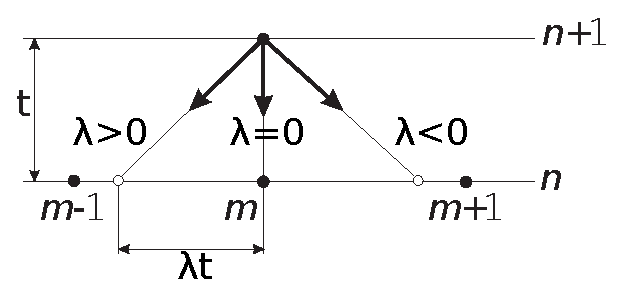
\includegraphics[width=0.5\textwidth]{eps/gcm-idea.eps}}
\caption{Принципиальная схема сеточно-характеристического метода.}
\end{figure}
Из точки пересечения характеристики со слоем $n$ значение $v_i$ переносится в 
точку $\xi^{n+1}_m$ путём решения \ref{advection_equation_final}:
$$v_i^{n+1}(\xi_m)=v^{n}_i(\xi_m-\lambda_i\tau) + {\tilde f}_i \tau.$$
Если характеристика не попадает точно в расчётный узел, то применяются различные
методы реконструкции значения в данной точке (в данной работе используется
интерполяция).
\subsubsection{Расщепление по пространственным направлениям}				
Идея метода \cite{fedorenko} решения исходной задачи состоит в расщеплении по трём пространственным координатам, то есть в разделении на этапе численного решения трёхмерной системы уравнений \ref{matrix_equation} на три одномерных,
\begin{equation}
\frac{\partial}{\partial t}\vec u+\mathbf{A}_x \frac{\partial}{\partial x}\vec u
= \vec f,
\label{matrix_equation_x}
\end{equation}
\begin{equation}
\frac{\partial}{\partial t}\vec u+\mathbf{A}_y \frac{\partial}{\partial y}\vec u
= \vec f,
\label{matrix_equation_y}
\end{equation}
\begin{equation}
\frac{\partial}{\partial t}\vec u+\mathbf{A}_z \frac{\partial}{\partial z}\vec u
= \vec f,
\label{matrix_equation_z}
\end{equation}
Эти уравнения решаются последовательно описанным в предыдущем параграфе методом с использованием
на каждом подшаге результатов, полученных на предыдущем подшаге.
\subsubsection{Расчёт граничных узлов}
Чистый метод характеристик, описанный выше, годится лишь для расчёта внутренних узлов
сетки, то есть только в том случае, если характеристика, выпущенная из узла, не
выводит за пределы области интегрирования. В случае, когда узел является
внешним, применяется иной подход для решения задачи. Рассматриваемая система
уравнений в граничных узлах области интегрирования имеет не больше трёх
\cite{chelnokov} выводящих характеристик, поэтому для корректной постановки
задачи требуется задание граничных условий для каждого внешнего узла сетки в
количестве, равном числу выводящих характеристик. Граничные условия могут быть
нескольких видов (символы без волны -- для первого тела, с волной -- для второго):
\begin{itemize}
\item{свободная граница
\begin{eqnarray}
\sigma_\tau=\sigma_n=0; \nonumber
\end{eqnarray}}
\item{скольжение тел друг относительно друга 
\begin{eqnarray}
v_n=\tilde{v}_n,\nonumber\\
\sigma_n=\tilde{\sigma}_n,\nonumber\\
\sigma_\tau=\tilde{\sigma}_\tau=0; \nonumber
\end{eqnarray}}
\item{слипание тел
\begin{eqnarray}
v_n=\tilde{v}_n,\nonumber\\
v_\tau=\tilde{v}_\tau.
\end{eqnarray}}
\end{itemize}
В случае, когда узел имеет выводящие характеристики, решение определяется
следующим образом: те компоненты искомого вектора $\vec{v}$, которые не имеют
выводящих характеристик, считаются при помощи сеточно"=характеристического
метода, описанного ранее; остальные уравнения заменяются граничными
соотношениями. После этого, решается полученная СЛАУ, из которой определяются
значения всех компонент вектора $\vec{v}$ в текущем узле.
\subsection{Пластический корректор}
В данной работе был реализован простейший корректор, реализующий нормировку вектора напряжений. Этот способ известен как правило корректировки Уилкинса, и верен только для идеальнопластической среды без упрочнения.

Рассчитанные в ходе эластичного предиктора напряжения в случае выхода за поверхность текучести --  $f(\sigma_{ij}) \geq 0$ (см. \ref{mizes}), приводятся на неё путём умножения на нормировочный коэффициент:
\begin{eqnarray}
s_{ij}^{n+1} = s_{ij}^e\frac{k_F}{J_2^e}	\\
J_2 = \sqrt{\frac{1}{2}s_{ij}s_{ij}}
\end{eqnarray} 